%preambulo
\documentclass[]{beamer}
\usepackage[spanish]{babel}
\usepackage[utf8]{inputenc}

%justificado
\usepackage{ragged2e}
\justifying

%tema
\usetheme{Warsaw}
\usecolortheme{default}
\setbeamercovered{transparent}

\title [Ingeniería en Software]{Personal Software Process - ISO/IEC 12207}
\author[Grupo 1]{Oscar León Trureo\\Sebastián Menéndez Sáez\\Claudio Piña Novoa}
\date{\today}
\institute[]{Universidad Tecnol\'ogica Metropolitana}
%\logo{}


%empieza el Documento
\begin{document}


\begin{frame}
	\maketitle
\end{frame}

\begin{frame}
	\frametitle{Outline}
	\tableofcontents[]
\end{frame}

\section{Personal Software Process}
		\subsection{Introducci\'on}
			\begin{frame}{Introducci\'on}
				Dentro del mundo del desarrollo en Software, podemos encontrar las metodolog\'ias, las cuales son un conjunto de buenas pr\'acticas, las cuales nos permiten:\\ \pause
				\begin{itemize}
					\item Crear mejores aplicaciones.\pause
					\item Llevar un mejor proceso de desarrollo.\pause
					\item Agilizar el desarrollo en sí.\pause
					\item etc \ldots
				\end{itemize}				
			\end{frame}
			
			\begin{frame}{Introducci\'on}
				Existen una gran cantidad de metodologías, las cuales pueden estar enfocadas al desarrollo en sí, a la gestión, a la calidad, al desarrollador, como también puede ser una mezcla.\\
				\smallskip
				Personal Software Process, es una metodolog\'ia enfocada a la calidad del desarrollo del software a nivel personal, la cual se basa en factores que veremos más adelante.
			\end{frame}						
			
		\subsection{Historia}
			\begin{frame}{Historia}
				\pause
				\begin{itemize}
					\item Creado en el año 1995 por Watt's S. Humphrey en la Universidad de Carnegie Mellon, en Pittsburgh, Pennsylvania.\\ \pause
					\item El primer curso fue imparti\'o en la Universidad de Carnegie Mellon.\\ \pause
					\item fue plasmado en el libro ``A Discipline for SW Engineering'' de Humphrey.\\
				\end{itemize}
			\end{frame}
		
				\begin{frame}
					\begin{quotation}``La calidad del software está dada por la cantidad de procesos usados para desarrollarlo y mantenerlo''.\end{quotation}
			
				\hfill -- \parbox[t]{.9\textwidth}{Watts S. Humphrey,
				\textit{Creador de Personal Software Process}}

				\end{frame}					
		
		\subsection{PSP}
			\begin{frame}{PSP}
				\textbf{Personal Software Process}, que en español significa \textbf{Proceso Personal de Software} (PSP), es un conjunto de buenas pr\'acticas las cuales se enfocan al control del tiempo y en la productividad de los Ingenieros en Software, ya sea en la mantencion de sistemas o en tareas de desarrollo.
			\end{frame}
			
			\begin{frame}{PSP}
				\textbf{PSP} no es un est\'andar, es m\'as bien un alternativa que permite mejorar la forma en la que se construye el software, pero con un enfoque ``individual'', por lo que es muy recomendada para los desarrolladores que estén interesados en mejorar en lo que llamamos ``desarrollo individual''.
				\begin{figure}
    				\scalebox{0.2}{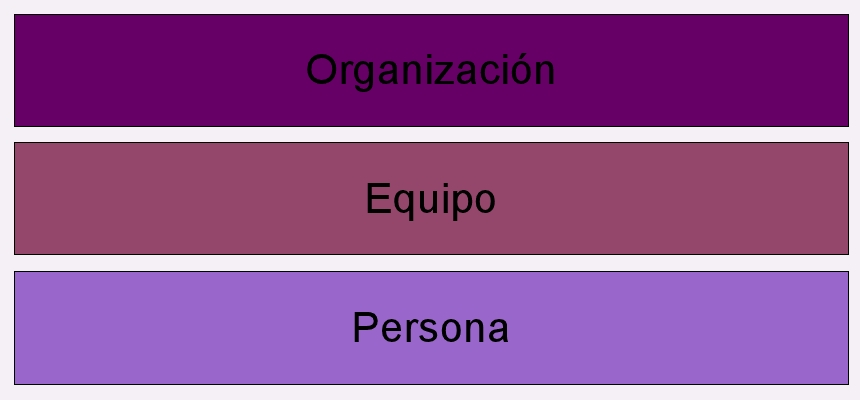
\includegraphics{Imagenes/Orga.jpg}} \caption{Niveles de la Organización}
				\end{figure}
			\end{frame}
				
\section{ISO/IEC 12207}
		\subsection{Introducci\'on}
			\begin{frame}{Introducci\'on}
				contenido introducción
			\end{frame}
		
		\subsection{Historia}
			\begin{frame}{Historia}
				contenido Historia
			\end{frame}
			
		\subsection{Desarrollo1}
			\begin{frame}{Desarrollo1}
				contenido Desarrollo1
			\end{frame}

		\subsection{Desarrollo2}
			\begin{frame}{Desarrollo2}
				contenido Desarrollo2
			\end{frame}
			
\section{Conclusi\'on}
	\begin{frame}{Conclusión}
		aqu\'i va la conclusi\'on
	\end{frame}				
			
\section{Bibliograf\'ia}
	\begin{frame}{Bibliograf\'ia}
		\begin{thebibliography}{9}
		
			%item 1		
			\bibitem{mo02} 
 			Victor M. Fleites Sabido 
 			\newblock {\em Personal Software Process}, 
 			\newblock http://www.slideshare.net/Tonymx/introduccion-a-personal-software-process.
		
			%item 2		
			\bibitem{sm-hin04} 
 			Armando David Espinoza Robles
 			\newblock{\em Metodologías de Desarrollo de Software}, 
 			\newblock http://www.slideshare.net/juliopari/4-clase-metodologia-de-desarrolo-de-software.
 			
		http://calidadesoftware.wordpress.com/2012/02/23/personal-software-process/ 			
		http://es.pdfsb.com/readonline/5a56464364516835575846394358706755554d3d-118608
 			
 		http://ingsw.ccbas.uaa.mx/sitio/images/material/psp.htm
		\end{thebibliography}
	\end{frame}

\end{document}